191. Прямоугольник ABCD разделили на четыре меньших прямоугольника с одинаковыми периметрами. Известно, что AB = 18 см, а BC = 16 см. Найдите длины сторон остальных прямоугольников. Обязательно объясните свой ответ.
\begin{center}
\begin{figure}[ht!]
\center{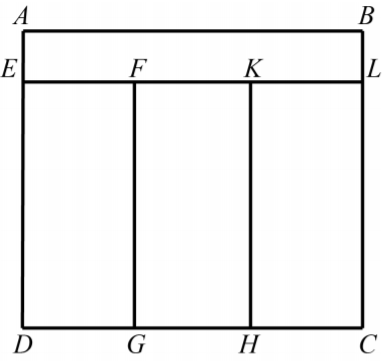
\includegraphics[scale=0.35]{41.png}}
\end{figure}
\end{center}
